\section{Bevezetés}

Az előző fejezetben bemutatásra került relációs adatbázisok sok pozitív tulajdonsággal rendelkeznek, ezért sok helyen és formában alkalmazzák őket, mivel a legtöbb a probléma megoldásához kiválóan használhatóak.
Azonban, mint a legtöbb rendszernél itt is szükséges kompromisszumokat kötni, hiszen rendelkeznek hátrányokkal is (\ref{subsect:reldbdisa}). A problémák nem érintenek minden alkalmazást, azonban vannak olyan alkalmazások, ahol nem egy relációs adatbázis a tökéletes megoldás. Az ilyen problémák megoldására jöttek létre a NoSQL adatbázisok.\nomenclature{NoSQL (not only SQL) adatbázis}{\hfill\\NoSQL adatbázisnak szokás nevezni, minden olyan adatbázist, amely eltér a relációs adatbázisoktól (flexibilis sorméretek, JOIN műveletek elhagyása, jó skálázhatóság). A NoSQL rendszerek legismertebb típusa a dokumentum-orientált adatbázisok, így a kifejezéseket szinonimaként is szokás használni.}
\hfill\\
Az első komolyabb adatbázis, amely szakított a klasszikus relációs megvalósítási formával, az 1989-ben megjelent Lotus Notes\footnote{Ma már IBM Lotus Notes, ugyanis 1995-ben az IBM megvásárolta Lotus céget} szerver oldali komponense a Lotus Domino volt. Természetesen már korábban is voltak próbálkozások, egészen pontosan az 1980-as években kifejlesztett BerkleyDB, vagy a szintén ekkor készült GT.M megoldás, de ezek nem tudtak elterjedni, illetve említésre méltó piaci részesedést elérni, ugyanis az 1980-as években sem az (adatbázist használó) alkalmazások száma nem volt magas, sem az alkalmazások nem igényeltek rugalmas adattárolási technikákat.
\hfill\\
A következő említésre méltó adatbázis-kezelő az 1997-ben elkészült Metakit volt, melyet az első dokumentum-orientált adatbázisnak is tartanak. A termék sikerességét mutatja, hogy az Apple Mac OS X termékében ezt használták a címjegyzék adatbázisának. A Metakit legutóbbi verziója 2007-ben jelent meg és a fejlesztői levelezőlistája még a mai napig aktív.

A ,,dotkomlufi'' kipukkanása a NoSQL adatbázisoknak is hatalmas lökést adott, melyet a következő felsorolás szemléltet:
\begin{description}
	\item{Memcached (2003)} \hfill \\
		\emph{Key-value (kulcs-érték)}, bárki számára ingyenesen használható adatbázis, amely a memóriában tárolja az adatokat, így biztosítva a rövid válaszidőket. Számos projektben használják átmeneti tárolóegységként (cache), ezáltal csökkentve az adatbázisrendszer terhelését, és az alkalmazás erőforrásigényét.\\
		Mivel a Memcached csak kulcs-érték adatbázis, így egyszerű adatstruktúrát érdemes benne tárolni. Szerializált szövegek használatával bonyolultabb struktúrák elhelyezése is megoldható, azonban ekkor le kell mondani a keresésről, és az indexelhetőségről.
	\item{Google BigTable (2004)} \hfill \\
		A Google saját fejlesztésű teljesen zárt adatbázisa, külső fejlesztőknek számára nem érhető el. Ma már a legtöbb Google termék ezt használja (Reader, Youtube, Mail, Maps).
	\item{Apache CouchDB (2005)} \hfill \\
		Az \emph{Apache Software Foundation}\nomenclature{Apache Software Foundation}{\hfill\\Az alapítvány open-source termékek fejlesztésével, a termékekhez kapcsolódó támogatás nyújtásával foglalkozik.\\Az alapítványhoz olyan termékek tartoznak, mint az Apache webszerver, a CouchDB vagy a Cassandra.} termékét a Lotus Notes ihlette adatbázis alapjaira fejlesztették, az igazi elterjedése az elmúlt két évben indult meg. A CouchDB-vel \aref{sec:couchdb} fejezet foglalkozik bővebben.
\end{description}
	
A következő időszakot, amelyet körülbelül 2005-től számítanak, a webes alkalmazások folyamatos térnyerése idézte elő. Ide tartozik a Google e-mail szolgáltatása, a GMail, a Twitter\nomenclature{Twitter}{\hfill\\Közösségi mikroblog szolgáltatás, segítségével a felhasználók maximum 140 karakterben tudnak egymásnak üzenni. \\Az oldalon már közel 200 millió hozzáférést regisztráltak. (\defcitealias{twitter_forbes}{Twitter Hits Nearly 200M Accounts, 2011}\citetalias{twitter_forbes})}, és a Facebook\nomenclature{Facebook}{\hfill\\Az egyik legismertebb közösségi oldal. 2011 áprilisában több mint 500 millió felhasználóval rendelkezett. (\defcitealias{fb_stat}{Facebook statisztika, 2011}\citetalias{fb_stat})}. Ekkor (2007) jelent meg, a mára komoly hírnevet kivívó adatbázis, a MongoDB, mely a későbbiekben részletesen bemutatásra kerül \aref{sec:mongodb} fejezetben. 2008-ban pedig a Facebook által nyílt forráskódúvá (open-source) tett Cassandra projekt vált elérhető a fejlesztők számára, amelynek fejlesztéséért szintén az Apache Software Foundation a felelős. A Cassandra-t kimagaslóan jó skálázhatóságának köszönhetően ma már a Facebook, és a Twitter is használja. A Cassandra skálázása és replikációja mögött a peer-to-peer technológia áll, ezáltal növelve az adatbázis rendelkezésre állási idejét.\\
2010-ben jelent meg a Membase, a Memcached klaszterekre szánt verziója, melynek segítségével akár egy több száz gépből álló szerverpark memóriája válik használhatóvá gyorsítótárazásra. 

\section{Miben más?}

A NoSQL adatbázisok létrejötte az \emph{új típusú} alkalmazások megjelenésének köszönhető. De mit is jelent az új típusú? A következő egyszerű példán keresztül kívánom bemutatni:\\
Adott szervezet honlapján az ügyfeleknek egy regisztrációs űrlapot kell kitölteniük, amelyen az ügyfél legfontosabb adatai (név, lakcím, születési dátum, fénykép, beszélt nyelvek) szerepelnek. Ezen adatok a szerveroldalon egy relációs adatbázisba kerülnek elmentésre. Ezzel idáig nincs is semmi probléma, az ügyfelek kitöltik, a cég pedig tud keresni, szűrni a kitöltött űrlapok között, illetve meg tudja tekinteni őket.\\
De mi történik, ha fel kell venni a mezők közé még egy plusz információt (telefonszám, Facebook-profil)? Amennyiben nincs erre felkészítve a rendszer, bár ha fel is van, nem lesz tökéletes az adatbázis-struktúra, ugyanis ebben az esetben a különböző mezők típusa vagy mindig szöveg, vagy rengeteg felesleges oszlop kerül az adatbázisba, hogy minden adat a neki megfelelő típusban legyen elmentve (szöveg, dátum, fájl). Tehát ha nincs felkészítve az adatbázis erre, akkor fel kell venni a kapcsolatot a honlapot készítő vállalattal, akiknek ki kell ezt javítani a honlapon, a szerver-, a kliensoldalon és az adatbázisban is, amely arányaiban véve nagyon sok idő. Ehhez a munkához szükség van legalább az adatbázisért felelős személyre, egy kliens- és egy szerveroldali programozóra. \\
Azonban mi történik, ha egy NoSQL adatbázis dolgozik a háttérben? Az eredeti feladat megoldása itt sem okoz komolyabb problémát, viszont ha ki kell egészíteni azzal a bizonyos plusz mezővel, könnyedén megtehető (az adatbázis módosítása nélkül), ugyanis nincs megkötve, hogy hány oszlopból kell állnia egy sornak, illetve milyen adattípus szerepelhet az adott oszlopokban (gyenge típusosság).\\
\\
Ezek után könnyen levonatható a tanulság, hogy milyen rendszerekben alkalmazható jól egy NoSQL adatbázis: folyamatosan módosuló adatszerkezeteknél, a felhasználók által testreszabható megoldásoknál, illetve az eltérő entitásokkal rendelkező adatstruktúráknál.
\\
Bár a dokumentum-orientált adatbázisok eme rugalmassága kényelmes megoldásnak tűnik a relációs adatbázisokhoz képest, azonban ezt már a legkorábbi key-value adatbázisok is könnyedén meg tudták oldani. A NoSQL adatbázisok valódi sikerének kulcsa azon a problémák a megoldásában rejtezik, melyet a mai modern alkalmazásfejlesztési problémák hoztak a felszínre:
\begin{description}
	\item{Teljes szöveges keresés (full-text search)} \hfill \\
		A teljes szöveges keresés lehetősége a legtöbb relációs adatbázisban megtalálható, azonban a fejlesztők ahol lehet, megpróbálják az adatkeresésnek ezt a módját elkerülni lassúsága miatt.
	\item{Az SQL nyelv} \hfill \\
		Az SQL nyelv bármennyire is beszélt nyelv közeli, egy komolyabb méretű adatbázisnál problémákat okozhat (erre jelenthet megoldást a \ref{ORM} fejezetben kifejtett ORM).\\
		Problémák forrása lehet, a tíz tábla feletti, szűréssel és aggregációval ellátott lekérdezések megírása és átlátása.\\
		SQL-ben nem jellemző, hogy a fejlesztők kommentekkel egészítenék ki az SQL mondatokat, amely szintén megértési problémát okozhat.
	\item{Geolokalizáció\nomenclature{Geolokalizáció}{\hfill\\Az internetre csatlakoztatott eszköz fizikai tartózkodási helyének meghatározása. Ez történhet a böngésző, vagy GPS segítségével.}} \hfill \\
		Ma már sok alkalmazás használ geolokalizációt, például a legtöbb közösségi hálózat (Facebook, Twitter), vagy éppen a webes térképszoftverek (Bing Maps, Google Maps).
	\item{Bináris fájlok tárolása} \hfill \\
		A legtöbb NoSQL adatbázist fájltárolási támogatással szállítják, amely szakít a relációs rendszerek bináris állományok tárolásának technikájával. A fájlok strukturáltan tárolódnak, általában szétdarabolva, a gyors elérés érdekében.
	\item{Horizontális, vertikális skálázhatóság} \hfill \\
		A horizontális skálázás a legtöbb relációs rendszerben megtalálható, ezt nevezik replikációnak\nomenclature{Replikáció}{\hfill\\A replikáció során a rekordok egy másik adatbázis szerveren is megjelennek, ez lehet az adatbázis töredéke, vagy egésze is. Ha az egyik (master) adatbázisba történik rekord beillesztés, az automatikusan megjelenik a többiben is.\\Az alkalmazások a replikációt a következőképpen szokták alkalmazni: az egyik adatbázisszervert kinevezik mester adatbázisnak, az adatok beszúrása ebbe történik, míg a többi kliens adatbázisként jelenik meg, azonban a kliensekbe nem történik rekord beszúrás, ezekből mindössze adatkiolvasás. Ezzel az adatbázis-konfigurációval csökkenthető a mester szerver terhelése, amely a költséges írási műveleteket végzi, miközben a gyakrabban történő kiolvasási műveletek a kevésbé leterhelt kliens adatbázisából történik.}, ilyenkor a kliens (\emph{slave}) vár a mester (\emph{master}) szerver üzenetére, hogy milyen változás történt az adatbázisban, amelyet a kliens is végrehajt.
		A vertikális skálázás is általában replikációval történik, azonban ez nem kliens-mester replikáció, hanem mester-mester, ahol minden szerver kliensként és mesterként is rész vesz a kommunikációban.
\end{description}

\section{Apache CouchDB}
\label{sec:couchdb}
	A CouchDB az Apache webszerver\nomenclature{Apache webszerver}{\hfill\\Az egyik legismertebb open-source, keresztplatformos webszerver. \\A projekt célja egy olyan webszerver kifejlesztése és karbantartása, amely biztonságos, hatékony és jól használható vállalati környezetben is. (\cite{apachewebserver})} fejlesztéséért is felelős Apache Software Foundation terméke. Az első verzió 2005-ben jelent meg. Az adatbázis felépítése erősen hasonlít a IBM Lotus Notes termékére, ugyanis a projekt vezető fejlesztője, Damien Katz, korábban a Lotus Notes fejlesztésében is részt vett.\\
	 Az információk tárolása adatbázisokban és dokumentumokban történik. Az adatok eléréséhez nincs szükség SQL tudásra, ugyanis JavaScript\nomenclature{JavaScript}{\hfill\\A JavaScript egy objektumorientált és funkcionális programozási nyelv, mellyel leginkább a böngészőben találkozni. A nyelv egyszerűségével és könnyen tanulhatóságával, ma már sok keresztfordítóban (cross-compiler) megtalálható.} segítségével végezhetők el a szűrések -amelyet nézetnek (view-nak) neveznek, egészen pontosan a MapReduce használatával.
	\subsection{Interfész}
		A CouchDB felépítése eltér a klasszikus adatbázisoktól. Az \ref{fig:conn_int_standard} ábrán egy olyan alkalmazás általános kapcsolódási interfésze látható, ahol az alkalmazás natív driverekkel (DLL fájl, vagy megosztott könyvtár) kapcsolódik az adatbázishoz.
		\begin{figure}[h]
			\centering
				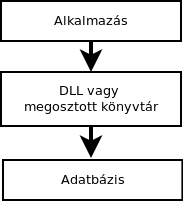
\includegraphics[scale=0.7]{pictures/conn_int_standard.png}%
				\caption{Példa egy általános kapcsolódási interfészre}
				\label{fig:conn_int_standard}
		\end{figure}
		
		A \ref{fig:conn_int_couchdb_expr} ábrán látható, ahogyan egy alkalmazás csatlakozhat a CouchDB-hez, itt azonban nincs szükség, semmilyen illesztőre, mindössze egy HTTP kliensre\nomenclature{HTTP kliens}{\hfill\\A legtöbb programozási nyelvben megtalálható osztály, melynek segítségével HTTP kérések indíthatók.}. Ennek az az előnye, hogy bármilyen programozási nyelvből indítható kérés az adatbázis felé. Hátránya viszont, hogy a lekérések nem lesznek olyan gyorsak, mint egy natív driver segítségével.
		\begin{figure}[ht]
			\centering
				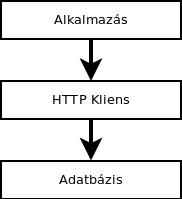
\includegraphics[scale=0.7]{pictures/conn_int_couchdb_expr.png}%
				\caption{Kapcsolódás CouchDB-hez szerver oldali rétegen keresztül}
				\label{fig:conn_int_couchdb_expr}
		\end{figure}
		\\
		\Aref{fig:conn_int_couchdb_simple} ábrán látható kapcsolódás már jobban megmagyarázza, miért jó a HTTP interfész. Ha egy weboldalt veszünk példának, akkor a kliens maga a böngésző lesz és szerveroldali programozási nyelv használata nélkül lehetségessé válik az információk megjelenítése. \\
		\hfill\\
		\clearpage
		\begin{figure}[ht]
			\centering
				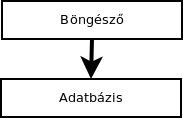
\includegraphics[scale=0.7]{pictures/conn_int_couchdb_simple.png}%
				\caption{A kliens közvetlen kapcsolódása az adatbázishoz}
				\label{fig:conn_int_couchdb_simple}
		\end{figure}
		\hfill\\
		\textbf{Miért jó ez?} \hfill \\
		Az egyszerű honlapoknál, a szerveroldali rész (legyen az PHP, ASP.NET vagy Perl) feladata mindössze annyi, hogy kapcsolódik az adatbázishoz, majd a lekérdezés eredménye alapján, felépíti a megfelelő HTML\nomenclature{HTML (HyperText Markup Language)}{\hfill\\A HTML egy leírónyelv, mely minden weboldal alapja. A böngészők a HTML oldal struktúrája alapján jelenítik meg a honlapokat.} oldalt. Ha lekerül HTML tartalom összeállításának terhe a szerverről, tehát kliensoldalon kerül felépítésre a tartalom, rengeteg erőforrás spórolható meg, ezáltal költséghatékonyabb szerver-üzemeltetés érhető el, így tulajdonképpen az ügyfél erőforrásaival fizet a szolgáltatás használatáért.\hfill\\
		Azonban ennek a technikának is van hátránya, mivel ami a weboldalaknál kliensoldalon (böngészőben) történik az bárki számára látható, ezért itt kiemelt szerepet kap a biztonság. Szerencsére a CouchDB nyújt lehetőséget a különböző adatbázisok jelszóval történő védelmére, illetve kívülről láthatatlanná tételére. Ilyenkor fontos, hogy csak azok az adatbázisok legyenek megtekinthetőek (kliensoldalról elérhetőek), amelyek nem tartalmaznak érzékeny információkat, például a regisztrált felhasználók vagy az adminisztrátorok személyes adatait.

		
		\subsubsection{A HTTP interfész}
			\label{subsect:couchdb_http}
			A CouchDB HTTP interfésze egy RESTful\nomenclature{RESTful (Representational State Transfer)}{\hfill\\A kliens és a szerver közötti adatkommunikáció lebonyolításának egyik lehetséges technikája. A HTTP/1.1 szabvány által definiált lehetőségekre épít, azaz nem csak GET kérésekkel kommunikál, hanem GET (lekérdezés), POST (létrehozás), PUT(létrehozás, frissítés), DELETE (törlés) kérésekkel.\\A weboldalakon gyakran alkalmazzák, ugyanis JavaScripttel végrehajtott AJAX (Asynchronous JavaScript and XML) kérésekben könnyebb az implementációja, mint más webszolgáltatásoknak (SOAP, RPC).} webszolgáltatás, mely jelentősen eltér a webszolgáltatások által korábban preferált SOAP\nomenclature{SOAP (webservice)}{\hfill\\A kliens és a szerver közti adatkommunikáció lebonyolítására használt protokoll. Az üzenetek XML formátumban kerülnek küldésre, melynek szigorú felépítése van, amit egy WSDL (Web Services Description Language) állomány ír le. } technikától. Itt ugyanis nem egy XML\nomenclature{XML (Extensible Markup Language)}{\hfill\\Az XML egy leírónyelv, az adatok strukturált tárolására.} fájl segítségével történik a webszerver utasítása, hanem standard HTTP kérésekkel.
			Dokumentumok lekérdezése GET-, egy adott dokumentum lekérdezése (az azonosítója megadásával) szintén GET kéréssel történik. A létrehozás POST, a frissítés PUT (azonosító megadása szükséges), míg a törlés DELETE (azonosító megadása szükséges) kérés küldésével hajtható végre. Megfigyelhető, hogy a kérések mennyire jól tükrözik a CRUD\nomenclature{CRUD (Create, Read, Update, Delete)}{\hfill\\Az adattárolás négy alapvető műveletének (írás, olvasás, frissítés, törlés) összefoglaló neve.} műveleteket.\\
		\hfill\\
		\textbf{Miért HTTP, és nem natív interfész?}
			A HTTP interfész nagy előnye, hogy ugyanazok az eszközök használhatók a performancia javítása érdekében, mint a webes alapú rendszereknél: terhelés elosztás (load-balancer\nomenclature{Load-balancer}{\hfill\\Magyarul terhelés elosztó. Nagy terhelés esetén a kiszolgálás nem egy rendszerről történik, hanem többről, ilyenkor a terhelés elosztó dönti el (egy adott algoritmus alapján), hogy melyik rendszer szolgálja ki a bejövő kérést.}), gyorsítótárak (cache\nomenclature{Cache}{\hfill\\A cache használatával, a több ugyanolyan kérésnél nem szükséges minden alkalommal elvégezni a számítási műveleteket, mert a gyorsítótárból azonnal kiszolgálható az előző (a jelenlegivel megegyező) kérésre adott válasz eltárolt változatával.}), SSL- és autentikációs proxy. Például a dokumentumok revíziós száma kiválóan használható ETag fejlécként\nomenclature{ETag fejléc (header)}{\hfill\\A weboldalaknál, kliensoldalon történő gyorsítótárazás egyik formája.\\A webszerverről érkező válaszok verziózására használják, ugyanis amíg kérésre adott válasz nem változik, az ETag fejléc értéke sem fog, így a böngésző le sem tölti. Új verzió esetén az ETag fejléc változik, ezáltal jelezve a böngészőnek az új tartalmat.} a cache szerveren.
	\\
	\subsection{Az adatmodell}
		\subsubsection{Dokumentum (Document)}
			\label{subsec:couchdbdocument}
			A CouchDB adatstruktúrájának legfontosabb része a dokumentum, amely megközelítőleg a relációs adatbázisok megadott táblája egy sorának feleltethető meg. Egy dokumentumban mezők találhatóak, melyek kulcs-érték formában jelennek meg. A kulcs bármilyen szöveg lehet, míg az érték a következők egyike:
			\begin{itemize}
				\item szöveg (string)
				\item egész szám (integer)
				\item lebegőpontos szám (float)
				\item dátum (JavaScript Date)
				\item objektumok (JavaScript object, Array)
			\end{itemize}
			Továbbá tartalmazhat hivatkozásokat más dokumentumra (URL-k), azonban nem kerül ellenőrzése a hivatkozás, illetve az adatbázis nem tartja fenn a konzisztenciát.
			\\
			A dokumentumok egymásba nem ágyazhatók.\hfill\\
			\\
			A \ref{fig:simple_couchdb_json} ábrán látható a dolgozat egy részlete CouchDB adatbázisban tárolva. A dolgozat címe, készítési ideje, és tartalma hasonlóan van tárolva, mint egy relációs rendszerben, azonban megfigyelhető, hogy míg egy relációs adatbázisban a címkékhez és a kommentekhez biztosan szükséges lenne egy kereszttábla beiktatása, itt egyszerűen egy tömbbel kifejezhető az egy a többes kapcsolatot.\\
			A dokumentum azonosítója ("\_id" mező) egy 128 bites, automatikusan generált érték (tehát a CouchDB egy adatbázisban maximum 3.4$^{38}$ dokumentumot tud tárolni). A revíziós szám is egy generált érték, azonban ez csak 32 bites, és egy hash függvény\nomenclature{Hash függvény}{\hfill\\Olyan matematikai algoritmus, amely a bemeneti (tetszőleges hosszúságú) adatot véges hosszúságúra képezi le. Digitális aláírásoknál és ellenőrző szövegeknél is alkalmazzák.} állítja elő. A revíziós szám használatával a dokumentum minden frissítésekor fizikailag egy új dokumentum jön létre. A lekérdezésekben a dokumentumnak mindig a legutolsó verziója látható. Tehát a revíziós szám, csak a dokumentumok különböző verzióinak megkülönböztetésére szolgál, illetve ennek segítségével oldja meg a tranzakciókat illetve replikációt is. (\defcitealias{couchdbdefguiderev}{Anderson et. al., 2010a}\citetalias{couchdbdefguiderev})
			\begin{figure}[ht]
				\centering
					\lstinputlisting[language=Javascript]{stuff/couchdb.json}
					\caption{Egy egyszerű CouchDB dokumentum}
					\label{fig:simple_couchdb_json}
			\end{figure}
			\\
			A dokumentumok szerializált JSON adatként kerülnek a lemezre.
		\subsubsection{Nézet (View)}
			\label{subsect:couchdbview}
			CouchDB-ben minden lekérdezést, csoportosítást, sorba rendezést nézetnek neveznek. \hfill\\
			\\
			A nézetek JavaScriptben írt függvények, amelyek nem tudják módosítani az adatbázisban tárolt adatokat, csak a elvégzik a szűrést (vagy csoportosítást, vagy éppen a sorba rendezést).\hfill\\
			A JavaScript függvények MapReduce alapúak, tehát minden függvénynek létezik egy \emph{map} és egy \emph{reduce} része. 
			\\
			\begin{figure}[ht]
				\centering
					\lstinputlisting[language=Javascript]{stuff/couchdb_map.js}
					\caption{A CouchDB Map függvénye}
					\label{fig:couchdb_map}
			\end{figure}

			\paragraph{\bf Map}
				A map függvénynek egy paramétere van, amely egy dokumentum, a függvényben itt végezhető az adott dokumentumra vonatkozó szűrés. A \ref{fig:couchdb_map} ábrán látható a CouchDB map függvénye használat közben, ahol a dokumentum címére történik a szűrés, tehát kijelenthető, hogy a map megfelel a relációs adatbázis szűrés (WHERE) záradékának.\\
				Amennyiben a cím megfelel a feltételnek, akkor átadásra kerül reduce függvénynek az \emph{emit} használatával. (\defcitealias{couchdbwiki}{Introduction to CouchDB Views, 2011} \citetalias{couchdbwiki})

			\begin{figure}[ht]
				\centering
					\lstinputlisting[language=Javascript]{stuff/couchdb_mapreduce.js}
					\caption{A CouchDB map és reduce függvénye}
					\label{fig:couchdb_map_expr}
			\end{figure}
			\hfill\\
			\paragraph{\bf Reduce}
				A Reduce függvény alkalmazása opcionális, segítségével aggregálható a map által szűrt információ. A \ref{fig:couchdb_map_expr} kódrészletben, az előző bekezdésben megismert map függvény látható más formában. Első paraméter itt a kommentelő neve lesz, a második pedig az egy, ezt megkapja a reduce és összesíti az egy névhez tartozó egyeseket, majd függvény visszaadja melyik kommentelő hány hozzászólást írt eddig.
		\hfill\\
		\subsection{Replikáció}
			A CouchDB replikációja hasonlóan működik, mint a relációs adatbázis rendszereké, lehetővé teszi az adatok megosztását az adatbázisok között.\\
			Viszont a replikáció indításához itt nincs szükség különböző konfigurációs fájlok írására, ugyanis egy POST kéréssel indítható illetve megszakítható (specifikálni kell a kérésben a forrás és a cél adatbázist), amely lehet egyszeri vagy folyamatos szinkronizáció. (\defcitealias{couchdb_repl}{CouchDB Replication, 2010}\citetalias{couchdb_repl})\\
			A replikáció indításkor az adatbázisok összehasonlításra kerülnek, majd a hiányzó adatok átkerülnek a céladatbázisba. A folyamat során csak azok a dokumentumok és mezők kerülnek át, melyek frissültek (\aref{subsec:couchdbdocument} fejezetben olvasható revíziós szám ebben nyújt segítséget). A szinkronizáció leállása (hálózati, vagy szoftveres hiba) esetén a replikáció attól a dokumentumtól folytatódik, ahol a leállás történt.
			
		\hfill\\
		\subsection{Tranzakciók}
			A CouchDB támogatja a tranzakciókat. A tranzakciók \aref{subsect:couchdb_http} fejezetben olvasható revíziós szám alapján történik. Azonban a CouchDB-ben található tranzakció nem egyezik a relációs adatbázisokban használttal. Itt ugyanis a tranzakciót, nem egy több lépésből álló műveletként kezelik, hanem az egyes műveletek számítanak egy tranzakciónak. \\Például, ha egy banki rendszerben átutalás történik, akkor az adott ügyfél számlájáról először leemelésre kerül az összeg, átkerül a folyamatban lévő átutalások közé, majd pedig arra a bankszámlára, amelyre a pénzt küldték. Ha ebben a folyamatban valami probléma történik (nincs elég pénz a számlán, nem lehetséges elindítani az utalást), akkor a tranzakció visszavonásával, minden visszaáll az eredeti állapotba. A CouchDB-ben ez azonban máshogy történik, mivel minden egyes lépés (a pénz leemelése, áthelyezése, elküldése) külön tranzakcióként hajtódik végre, ezért nem lehet egyben visszavonni hiba esetén. Viszont a tranzakciók egyesével, egy ellenirányú tranzakció létrehozásával visszavonhatóak. (\defcitealias{couchdbdefguidetrans}{Anderson et. al., 2010b}\citetalias{couchdbdefguidetrans})
	\hfill\\\hfill\\
	Bár a CouchDB már 2005 óta elérhető a nagyközönség számára, a valódi felfutása 2009 és 2010 közt indult meg. Azóta már olyan cégek használják mint a svájci székhelyű Nukleáris Kutatások Tanácsa, a CERN\footnote{CERN (Conseil Européenne pour la Recherche Nucléaire): a Nukleáris Kutatások Európai Tanácsa}, ahol évente az adatbázisba körülbelül 10 petabájt információ kerül be. (\defcitealias{couchdbcern}{CERN, 2010}\citetalias{couchdbcern})\\
	A CouchDB már rendelkezik saját hoszting szolgáltatóval, ez a CouchBase, amely a CouchDB-t ötvözte a Membase szolgáltatásaival, ezáltal csökkentve válaszidőket, az adatbázis terhelést és növelve a szolgáltatásfolytonosságot A szolgáltatás minőségét jól jellemzi, hogy a CERN mellett már nagy cégek is használják, mint a BBC, a PayPal, a Adobe és a Vodafone.
\section{MongoDB}
\label{sec:mongodb}
	
	A MongoDB egy dokumentum-orientált adatbázis, a 10gen Inc. cég terméke. A fejlesztés célja az volt, hogy egy skálázható kulcs-érték adatbázist hozzanak létre, amely kiválóan megoldja, a gyakran felmerülő problémákat az alkalmazások fejlesztésében.\\
	A MongoDB-t egyre szívesebben választják komoly felhasználói bázissal rendelkező szolgáltatások, amelyek közül vannak, akik a korábbi relációs adatbázis rendszereiket teljesen lecserélik, vannak akik párhuzamosan használják a két rendszert, kiaknázva az erősségeiket. 2011-re olyan cégek döntöttek a MongoDB mellett, mint az open-source szoftverek gyűjtőhelye a Sourceforge.net, a foursquare közösségi oldal, vagy éppen a New York Times.
	
	\subsection{Interfész}
		A MongoDB kapcsolódási interfésze megegyezik a relációs adatbázisoknál használt technikával, azaz natív driverekkel lehet kapcsolódni, bár szükség esetén kiegészíthető RESTful webszolgáltatás bővítménnyel.\\
		Az adatbázishoz vagy valamilyen támogatott programozási nyelv, vagy a szerverkomponens mellé települő konzolos kliens  segítségével lehet hozzáférni. A MongoDB-hez hivatalosan támogatott grafikus felülettel ellátott adatbázis-kezelő nem készült még, azonban a felhasználók által készített kliensprogramok között már találunk ilyet. Ezek minőségével és használhatóságával vannak problémák, így a következő példák is konzol segítségével készültek.\\
		A konzol elérhető a MongoDB által támogatott platformokon (Windows, OS X, Linux, Solaris), Windows operációs rendszeren a parancssorba, míg Linuxon a terminálba beírva a \emph{mongo} parancsot.
		\hfill\\
		A konzolban néhány kivételtől eltekintve (adatbázis létrehozás, listázás) az utasítások JavaScript függvények.\hfill\\
		A \ref{fig:mongodbcreate} ábrán látható egy adatbázis létrehozása, ahol mindössze a \emph{use <név>} utasítás kiadásával, már létre is jött az adatbázis.
		\\
		\begin{figure}[ht]
			\centering
				\lstinputlisting[language=Javascript]{stuff/mongodb_create.js}
				\caption{Adatbázis létrehozása MongoDB-ben}
				\label{fig:mongodbcreate}
		\end{figure}
		\\
			\Aref{fig:mongodbcreate} ábrán látható kifejezés lefuttatása után, az adatbázis a \emph{db} változó segítségével férhető hozzá, ezáltal megkönnyítve a programozó dolgát, a lekérdezés megírásakor az adatbázis nevének begépelésétől.\\
		A gyűjtemény létrehozása sem sokkal bonyolultabb, mint az látható \aref{fig:mongodbcreatecoll} ábrán, a \emph{createCollection( <név>, { <opcionális paraméterek> } )} parancs kiadásával jön létre az adott adatbázisban.\\

		\hfill\\
		\begin{figure}[ht]
			\centering
				\lstinputlisting[language=Javascript]{stuff/mongodb_create_coll.js}
				\caption{Gyűjtemény létrehozása MongoDB-ben}
				\label{fig:mongodbcreatecoll}
		\end{figure}
		\\
		
	\subsection{Az adatmodell}
		A MongoDB felépítése hasonlít a relációs adatbázisok adatszerkezetére, vannak adatbázisok, amelyek gyűjteményeket (Collections) tartalmaznak. A gyűjtemények megfeleltethetőek a relációs adatbázisok tábláinak, amelyek tartalmazzák az adatsorokat. Egy adatbázis több gyűjteménnyel is rendelkezhet.
		Nagy különbség a többi adatbázishoz képest, hogy ha itt egy új sor kerül beszúrásra, és az adatbázis vagy a gyűjtemény nem létezik még, akkor automatikusan létrehozásra kerül, a konfigurációban megadott paraméterekkel, sőt alapértelmezetten automatikus indexeléssel.\\
		A gyűjtemények dokumentumokból épülnek fel.
		
		\subsubsection{Dokumentum}
			MongoDB-ben a dokumentum hasonló szerepet tölt be mint a CouchDB-nél (\ref{subsec:couchdbdocument}), itt is az adatmodell legalsó rétege. \Aref{fig:mongodbsimple} ábrán látható egy dokumentum. Megfigyelhető, hogy az adat itt is JSON formátumban jelenik meg, valójában ez azonban BSON\nomenclature{BSON (Binary JSON)}{\hfill\\A BSON felépítése megegyezik a JSON felépítésével, azonban itt nem csak a JSON specifikációban megadott adattípusok fordulhatnak elő, hanem egy BinData objektum, amelyben bináris fájlokat lehet tárolni.}, ugyanis az adatbázis a bináris fájlokat is ebben a struktúrában tárolja, és a JSON formátum specifikációja (\defcitealias{jsonspec}{ECMAScript, 2009}\citetalias{jsonspec}) nem ad lehetőséget bináris adatok tárolására.\hfill\\
			A dokumentumok mérete maximum 4 kilobájt lehet.
			
			\begin{figure}[ht]
				\centering
					\lstinputlisting[language=Javascript]{stuff/mongo.json}
					\caption{Egy egyszerű MongoDB dokumentum}
					\label{fig:mongodbsimple}
			\end{figure}
			
			\begin{figure}[ht]
				\centering
					\lstinputlisting[language=Javascript]{stuff/mongodb_create_doc.js}
					\caption{Dokumentum létrehozása MongoDB-ben}
					\label{fig:mongodbcreatedoc}
			\end{figure}
			\newpage
			\flushleft
			Egy dokumentum létrehozása látható \aref{fig:mongodbcreatedoc} ábrán. \\
			A MongoDB dokumentumokban a következő adattípusok tárolhatók:
			\begin{itemize}
				\item igaz/hamis értékek (boolean)
				\item egész számok (integer)
				\item lebegőpontos számok (double)
				\item szöveg (string)
				\item dátum (JavaScript Date)
				\item reguláris kifejezések (JavaScript RegExp-ek)
				\item objektumok (JavaScript object, Array)
				\item üres értékek (null)
				\item id (ObjectID)
			\end{itemize}
		\subsubsection{Lekérdezések}
			A MongoDB-ben történő lekérdezések alapja is a MapReduce, akárcsak a CouchDB-nél (\ref{subsect:couchdbview}). Itt azonban a CouchDB-vel ellentétben, nem kell megírni minden egyes szűrést vagy keresést végző map és reduce függvényt, ugyanis az adatbázisban megtalálható beépítve sok hasznos szűrési és aggregációs függvény. Viszont, az optimalizált keresések érdekében, természetesen futtatható a saját map és reduce is. \\
			\hfill\\
			\Aref{fig:mongodbfind} ábrán látható egy lekérdezés, amely a következőket hajtja végre:
			\begin{itemize}
				\item leszűri azokat a sorokat, amelyeknél létezik \emph{dbTípus} kulcs és az értéke ráillik a \emph{mongodb} reguláris kifejezésre, \nomenclature{Reguláris kifejezés}{\hfill\\A reguláris kifejezés segítségével, olyan szabályok hozhatók létre, melyekkel a szövegekben (a szabályok alapján) lehet keresni.} eltekintve a kis és nagybetűktől (SQL WHERE záradék)
				\item száz darabra csökkenti a sorok számát (SQL LIMIT záradék)
				\item az első húsz dokumentum kihagyásra kerül, és a huszonegyediktől választ ki száz darabot (SQL LIMIT vagy OFFSET záradék)
				\item a leszűrt dokumentumokat sorba rendezi, \emph{létrehozva} mező alapján csökkenő sorrendben (SQL ORDER BY DESC záradék)
			\end{itemize}
			
			\begin{figure}[ht]
				\centering
					\lstinputlisting[language=Javascript]{stuff/mongodb_find.js}
					\caption{Keresés MongoDB-ben}
					\label{fig:mongodbfind}
			\end{figure}
	\subsection{Fájltárolás}
		A MongoDB-ben egyik szolgáltatása a \emph{GridFS}. A GridFS felelős a fájlok tárolásáért az adatbázisban. Ha MongoDB-be beszúrásra kerül egy fájl, akkor először az adatbázis szétdarabolja szeletekre (chunk), melyek dokumentumokként kerülnek eltárolásra, a szeletek maximális mérete 4 megabájt lehet.\\
		A fájlok és a fájlok részei külön gyűjteményekbe kerülnek. \Aref{fig:mongodbmasterfile} ábrán látható egy eltárolt, közel 165 megabájtos zenefájl. A dokumentumban látható a fájl mérete, a neve, az MD5 hash\nomenclature{MD5 hash}{\hfill\\Az MD5 hash 128 bites egyirányú kódolási algoritmus.} értéke, a feltöltése ideje és az eltárolt szeletek mérete. A fájl szeleteinek mérete 262 148 bájt azaz az adott fájl 659 részletben van eltárolva.
		\begin{figure}[ht]
				\centering
					\lstinputlisting[language=Javascript]{stuff/mongodb_masterfile.json}
					\caption{Egy MongoDB-ben eltárolt fájl}
					\label{fig:mongodbmasterfile}
		\end{figure}
		\newpage
		\Aref{fig:mongodbfile} ábrán az első szelet dokumentuma látható, amely rendelkezik egy fájl azonosítóval ("files\_id" mező, mely megmutatja melyik fájl része az aktuális dokumentum), egy számmal, hogy hányadik szelet ("n") és egy adat résszel ("data"), mely tartalmazza a bináris adatot.
		\\
		\begin{figure}[ht]
				\centering
					\lstinputlisting[language=Javascript]{stuff/mongodb_file.json}
					\caption[DUMMY]%
					{\Aref{fig:mongodbmasterfile} ábrán látható fájl egy része (chunk)}
					\label{fig:mongodbfile}
		\end{figure}
		\hfill\\
		\textbf{Miért ilyen a tárolás?}
		\hfill\\
		Ennek a tárolási módszernek az az előnye, hogy ha a webes alkalmazásban, ahol zenéket lehet hallgatni, a felhasználó a 3. perctől kívánja ezt megtenni, akkor nem kell az adatbázistól elkérni az egész fájlt, mindössze attól a szeletettől kell lekérdezni, amelyet valóban hallgatni akar a felhasználó.\\
		Továbbá, ha az adatbázisban 30-40 gigabájtos fájlok tárolása történik, amelyeket a felhasználók le akarnak tölteni, akkor a relációs adatbázisban az egész fájlt le kell kérdezni, melyet az alkalmazás megpróbál betölteni a memóriába, viszont ha a szerver nem rendelkezik ennyi memóriával, akkor nem tudja visszaadni a felhasználónak.
		\newpage
		 MongoDB-ben a 30-40 gigabájtos fájlnál sem fordulhat ilyen elő, mert ha az egész fájlt kéri el az alkalmazás, akkor is mindig csak egy szeletet ad át az adatbázis, azaz a memóriában maximum 4 megabájt lesz lefoglalva.
	\subsection{Replikáció}
		A MongoDB támogatja az aszinkron replikációt automatikus helyreállítással (hálózati vagy szerverhiba esetén). A replikációnak két fajtája van: mester-kliens, és a replica set alapú.
		
		\subsubsection{Mester-kliens}
			A mester-kliens általában egy mester adatbázisból és egy (\ref{fig:mongodb_repl_m_s} ábra) vagy több (\ref{fig:mongodb_repl_m_sss} ábra) kliensből áll. Az egyetlen mester adatbázisba történik az adatok beszúrása, melyek automatikusan bekerülnek a kliens(ek) adatbázisába (a master egy olvasási eseményt küld a klienseknek). Amennyiben a kliensek kiesnek a replikációban (ez történhet az adatbázis szerver újraindulása miatt, hálózati forgalom hibáiból), a kliensek automatikusan újraszinkronizálják magukat.\\
			Azt, hogy egy szerver mester vagy kliensként vesz részt az adattárolásban, a konfigurációban megadott érték dönti el. \\
			A kliensek irányába történő szinkronizáció letiltható a mester szerverről, az adott kliens címének kizárásával.\\
			
			\begin{figure}[ht]
				\centering
					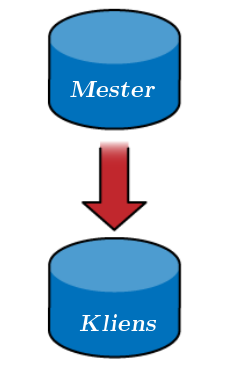
\includegraphics[scale=0.5]{pictures/mongo_repl_m_s.png}%
					\caption[DUMMY]%
					{Egy mester, egy kliens replikáció a MongoDB-ben (\cite{scaling_mongodb_repl_m_s})}
					\label{fig:mongodb_repl_m_s}
			\end{figure}
			
			\begin{figure}[ht]
				\centering
					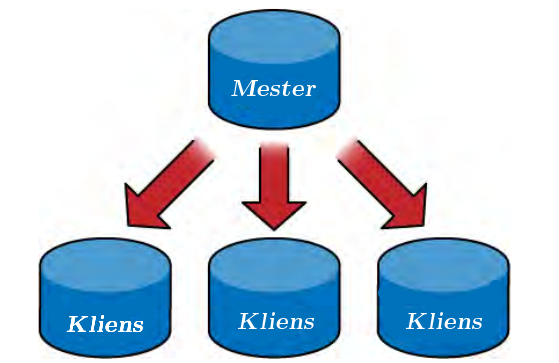
\includegraphics[scale=0.5]{pictures/mongo_repl_m_sss.png}%
					\caption[DUMMY]%
					{Egy mester, három kliens replikáció a MongoDB-ben (\cite{scaling_mongodb_repl_m_sss})}
					\label{fig:mongodb_repl_m_sss}
			\end{figure}
		\hfill\\
		\subsubsection{Replica set}
			A replica set tulajdonképpen egy mester-kliens replikáció automatikus helyreállítással. Ez azt jelenti, hogy a kommunikációban továbbra is egy mester (elsődleges) és egy kliens (másodlagos) szerver áll rendelkezésre, azonban hiba esetén a kliens mesterré válik, és a rekord beillesztések az új mester szerverbe folytatódnak. Amennyiben az eredeti mester helyreáll, az adatszinkronizáció elkezdődik, majd a végeztével minden visszaáll az eredeti állapotba, azaz az elsődleges szerver lesz ismét a mester, míg másodlagos klienssé válik.\\
			A rendelkezésre állás tovább fokozható másodlagos szerverek priorizálásával (\ref{fig:mongodb_repl_set} ábra).\\
			\begin{figure}[ht]
				\centering
					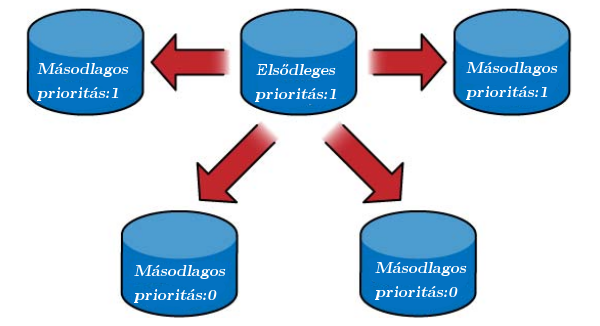
\includegraphics[scale=0.5]{pictures/mongodb_repl_set.png}%
					\caption[DUMMY]%
					{Replica set egy lehetséges felépítése a MongoDB-ben (\cite{scaling_mongodb_repl_set})}
					\label{fig:mongodb_repl_set}
			\end{figure}
			\newpage
			A szerverek ebben az esetben lehetnek akár klaszterek is, melynél az egész elsődleges klaszter kiesése után a legnagyobb prioritású másodlagos klaszter veszi át a mester szerepet, és így tovább egészen az utolsó működőképes szerverig vagy klaszterig.

			Az elsődleges szerver kiesése után a MongoDB, a következő legmagasabb prioritású szervert választja, amennyiben egynél több ilyen van, akkor a legutolsó szinkronizáció óta eltelt idő alapján választ (\ref{fig:mongodb_repl_set_failover} ábra).
	
			
			\begin{figure}[ht]
				\centering
					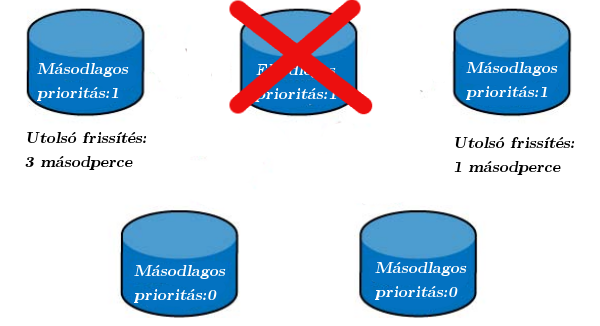
\includegraphics[scale=0.5]{pictures/mongodb_repl_set_failover.png}%
					\caption[DUMMY]%
					{Döntéshozatal replica set replikációnál a MongoDB-ben, az elsődleges szerver hibája esetén (\cite{scaling_mongodb_repl_set_failover})}
					\label{fig:mongodb_repl_set_failover}
			\end{figure}
	\subsection{Tranzakciók}
		A MongoDB nem MVCC\nomenclature{MVCC (Multversion Concurrency Control)}{\hfill\\Adatbázisoknál használt technika. Az adatbázis törlés esetén valójában nem töröl, csak törlésre jelöli az adott sort, illetve rekord frissítés esetén az adott rekord nem felülírásra kerül, hanem készül belőle egy újabb verzió. \\Az MVCC-t használó rendszerek nagy előnye, hogy könnyen vissza lehet állítani az adatokat egy korábbi verzióra.}, hanem helyben-frissítés (update-in-place) alapú adatbázis-kezelő rendszer. A tranzakciók hiánya miatt a MongoDB használata elképzelhetetlen pénzügyi rendszerekben, viszont olyan alkalmazásoknál, ahol másodpercenként több száz vagy ezer rekordot kell létrehozni, lekérdezni, frissíteni vagy törölni a helyben-frissítés jobb választás lehet, ugyanis így kisebb az esélye a hibák felmerülésének a replikációkban. (\defcitealias{mongodb_vs_couchdb}{Comparing MongoDB and CouchDB, 2011}\citetalias{mongodb_vs_couchdb})
